%!TEX root = main.tex

\chapter{Introducción}

La web actual está hecha por y para las personas. Desde las publicaciones en las
redes sociales hasta los artículos más avanzados en las enciclopedias virtuales
son formas de transferir información entre individuos y por ello utilizan el
lenguaje natural para hacer más fácil su entendimiento. Si bien estas
características facilitan la comprensión para el ser humano, hacen cada
vez más difícil el manejo de estos datos por parte de las computadoras debido a
la falta de un lenguaje común, lo que las obliga a intentar interpretar el
contexto y la intencionalidad del emisor, todo esto sumado a la masividad de la
información publicada hoy en día, donde todos pueden publicar lo que quieran y
en cualquier formato.

La Web Semántica nace como forma de solucionar esta problemática.
Su objetivo es que las maquinas puedan generar e intercambiar datos por Internet 
de manera que estos sean interpretables y procesables de forma simple tanto por
las personas como por otras computadoras.
Esto implica que los datos deben tener un modelo común, compatible y general,
y además, una visualización acorde para facilitar la lectura de los mismos por
los seres humanos.

Uno de los pilares fundamentales para la creación de una web en la cual toda
información pueda ser accedida por computadores de manera rápida y efectiva es
la generación de datos enlazados, es decir, la publicación e integración del 
conocimiento existente a un modelo que permita la interconexión y extensión de
los datos sin limitar el dominio ni las relaciones de los mismos.

Tim Berners-Lee, el inventor de la web y un propulsor de la Web Semántica,
a través de el \emph{World Wide Web Consortium}, ha generado estándares que
ayudan a solucionar este problema como son RDF, SPARQL entre otros.
Además, propone una clasificación de cinco estrellas para los datos publicados:
\begin{enumerate}
  \item
    Publica tus datos en la web, con cualquier formato y una licencia abierta.
  \item
    Utiliza datos estructurados (tablas, antes de imágenes de las mismas, etc).
  \item
    Utiliza formatos no propietarios.
  \item
    Utiliza URIs para denotar las cosas de manera que la gente pueda apuntar a
    ellas\footnote{
    Una forma de hacerlo es con URL, links a paginas web por ejemplo, de manera
    que otras personas puedan revisar el contenido y enlazar con él.}.
  \item
    Enlaza tus datos con otros para proveer contexto.
\end{enumerate}

Siguiendo los estándares y las recomendaciones hechas por Tim Berners-Lee se han
creado variados proyectos.
Actualmente existe una gran cantidad de datos de libre acceso enlazados en la
web. La figura \ref{fig:cloud} muestra un esquema de ellos y provee una visión
global de los diferentes tópicos que estos datos tratan, ya sean datos
geográficos, de redes sociales, biológicos o lingüísticos (entre otros).

En este trabajo nos enfocaremos en los datos biológicos, en particular a partes
del proyecto Bio2RDF.
Dicho proyecto (en su \emph{release} 3) incorpora la información de 35 bases de
datos RDF con información biológica, cerca de 11.000 millones de triples que
conforman la red de data enlazada más grande de esta ciencia.

En trabajos anteriores como en Hu \emph{et al.}\cite{hu2015link} se han
determinado parámetros como el grado de distribución, la simetría y la
transitividad de los enlaces entre las diferentes bases de datos que lo
componen, además de la existencia del fenómeno conocido como ``mundo pequeño'',
lo que significa que, a pesar del gran número de nodos que existen en esta red
de datos, generalmente es posible encontrar un camino relativamente corto entre
ellos.

Pero, ¿Cuales son los datos más importantes para los usuarios?, ¿Cómo se
relacionan entre ellos? Son interrogantes que se presenta naturalmente al
momento de evidenciar la cantidad abrumadora de datos enlazados existentes.
Es ente trabajo responderemos dichas interrogantes para parte de los datos de
Bio2RDF, en especifico la base de datos DrugBank, la cual no solo es de las más
consultadas del proyecto, sino que además posee algunos de los datos más
interesantes de esta ciencia como son los medicamentos.

\begin{figure}[ht]
  \centering
  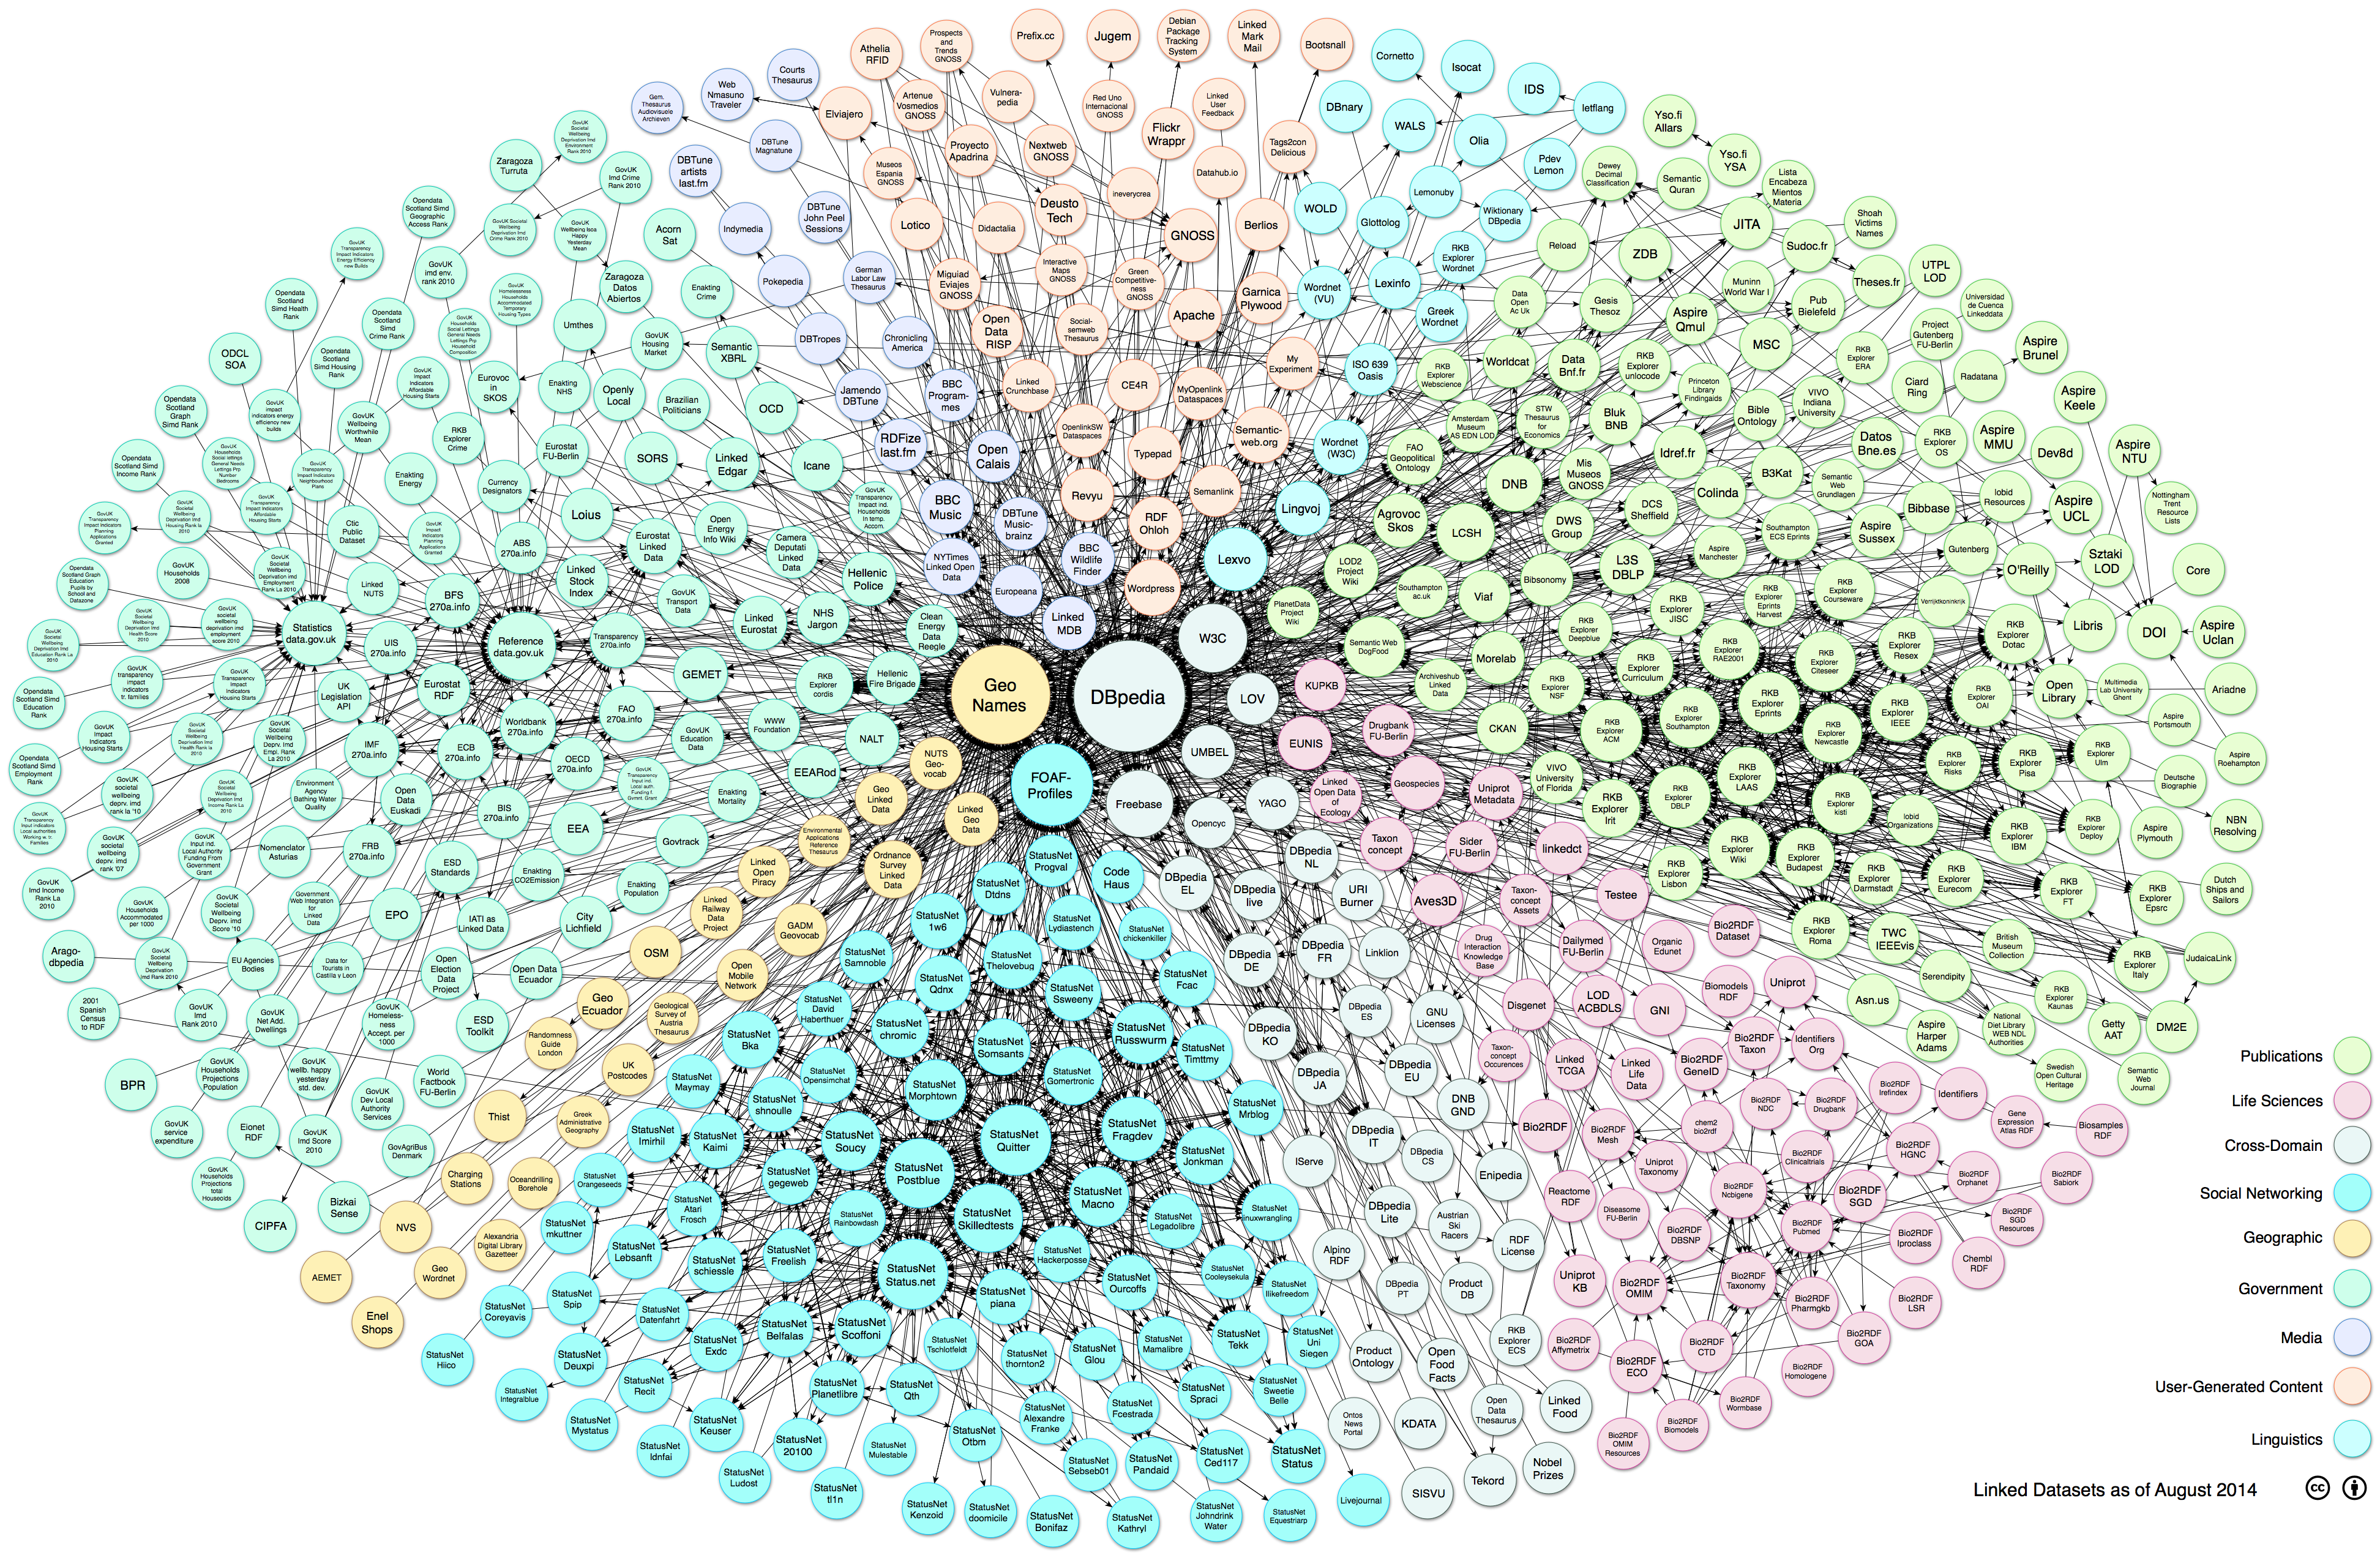
\includegraphics[width=\textwidth]{figures/open_linked_data_could.png}
  \caption{Conexiones entre las bases de datos abiertas hasta agosto del 2014.}
  \vspace{-.2cm}
  \caption*{En morado las bases de datos biológicas, gran parte de ellas son
  parte del proyecto Bio2RDF. Creado por Linked Open Data Cloud project\cite{lod:cloud}.}
  \label{fig:cloud}
\end{figure}
~\vspace{-1cm}

\section{Identificación del problema}
Debido al volumen de datos que se manejan en el proyecto Bio2RDF se vuelve
interesante determinar cual es la información más importante consultada por
parte de los usuarios y así verificar el soporte que ésta tiene en el modelo. 
Para ello es indispensable contar con métricas que analicen el uso de los datos
consultados, la relevancia y la relación entre los mismos.

Actualmente no existe un estudio que determine cual es el subconjunto de datos
que realmente son son utilizados y por ello no es posible verificar cuales son
las entidades más importantes dentro de este proyecto.

Además sabemos que el fenómeno de ``mundo pequeño'' que presenta Bio2RDF, es
generalmente evidenciado en las redes sociales. En estas se 
teoriza que dos individuos cualquiera están relacionados entre si por un número
pequeño de pasos, como describe la hipótesis de los seis grados de separación o
muestra el estudio ``Anatomy of Facebook''\cite{ugander2011anatomy}.

Esta característica evidencia la existencia de individuos claves en la
comunicación de una red social. 
Una de las métricas más utilizadas y con mejores resultados para determinar
estos individuos es el análisis de centralidad.

La centralidad es una forma de medir la importancia de un nodo en una red.
En las redes sociales se transforma en una medida de la influencia de una
persona con respecto a sus pares, en redes de transporte puede identificar los
puntos críticos y cuellos de botella, y de la misma manera, en una red RDF
esperamos que señale los datos más importantes.

Debido a estas características consideramos atractivo generar un cálculo de
centralidad para los datos consultados por los usuarios al proyecto Bio2RDF,
específicamente a una de las bases de datos que presenta mayor cantidad de
consultas en él: DrugBank, y de esta manera identificar tanto cuales son las
instancias más importantes como las relaciones claves existentes en ella.

\section{Objetivos}

El objetivo de este trabajo es generar estadísticas de centralidad sobre el
subconjunto de datos consultados por los usuarios a la base de datos DrugBank,
parte importante del proyecto Bio2RDF.
Se espera lograr determinar cuales son los miembros claves de esta base de datos
y verificar si los resultados son congruentes con el modelo de datos planteado
por el proyecto.

\subsection{Objetivos específicos}
Para el logro del objetivo general se plantean los siguientes objetivos
específicos:
\begin{enumerate}
  \item
    Generar un subgrafo del proyecto Bio2RDF a través del análisis de las
    consultas SPARQL hechas al servidor por parte de los usuarios en un periodo
    de tiempo determinado.
  \item
    Analizar el grafo generado por medio de métricas de centralidad para grafos.
  \item
    Comparar los resultados del estudio con el proyecto Bio2RDF.
\end{enumerate}
